\documentclass{ximera}

\newcommand{\RR}{\mathbb R}
\renewcommand{\d}{\,d}
\newcommand{\dd}[2][]{\frac{d #1}{d #2}}
\renewcommand{\l}{\ell}
\newcommand{\ddx}{\frac{d}{dx}}
\newcommand{\dfn}{\textbf}
\newcommand{\eval}[1]{\bigg[ #1 \bigg]}


\author{Jim Talamo and Bart Snapp}
\license{Creative Commons 3.0 By-bC}


\outcome{}


\begin{document}
\begin{exercise}

Suppose that $\{a_n\}_{n=1}$ is an \emph{geometric} sequence, whose first few terms are shown below:

\[
\frac{3}{5}, \frac{-3}{25}, \frac{3}{125}, -\frac{3}{625}, \frac{3}{3125}, \ldots
\]

Note that since we are told that the sequence is geometric:

\begin{multipleChoice}
\choice{The difference between subsequent terms is constant.}
\choice[correct]{The ratio of subsequent terms is constant.}
\end{multipleChoice}

In fact, the ratio between successive terms is $\answer{-\frac{1}{5}}$:

\begin{exercise}

  \begin{image}
    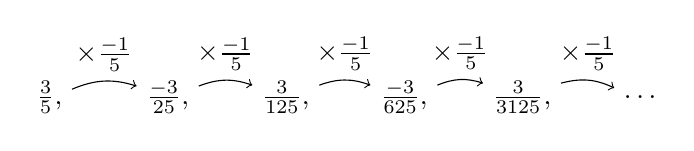
\begin{tikzpicture}[node distance=1.5cm]
    \node (a1) {$\frac{3}{5}$,};
    \node (a2) [right of=a1] {$\frac{-3}{25}$,};
    \node (a3) [right of=a2] {$\frac{3}{125}$,};
    \node (a4) [right of=a3] {$\frac{-3}{625}$,};
    \node (a5) [right of=a4] {$\frac{3}{3125}$,};
    \node (a6) [right of=a5] {$\ldots$};

    \path[->] (a1) edge [bend left=20] node[above] {$\times\frac{-1}{5}$} (a2);
    \path[->] (a2) edge [bend left=20] node[above] {$\times\frac{-1}{5}$} (a3);
    \path[->] (a3) edge [bend left=20] node[above] {$\times\frac{-1}{5}$} (a4);
    \path[->] (a4) edge [bend left=20] node[above] {$\times\frac{-1}{5}$} (a5);
    \path[->] (a5) edge [bend left=20] node[above] {$\times\frac{-1}{5}$} (a6);
  \end{tikzpicture}
  \end{image}
  This sequence can be described both explicitly and recursively.
  
  It is given by the explicit formula $a_n=\answer[given]{\left(\frac{3}{5}\right)\cdot
    \left(\frac{-1}{5}\right)^{n-1}}$ for $n \geq 1$.
    
    It is given by the recursive rule $a_1 = \answer[given]{\frac{3}{5}}$ and
  $a_{n+1} = \answer[given]{\left(\frac{-1}{5}\right)}\cdot a_n$. 
  
\end{exercise}
\end{exercise}
\end{document}
